\documentclass[aspectratio=169]{beamer}

\mode<presentation> {
%\usetheme{default}
%\usetheme{AnnArbor}
%\usetheme{Antibes}
%\usetheme{Bergen}
%\usetheme{Berkeley}
%\usetheme{Berlin}
%\usetheme{Boadilla}
%\usetheme{CambridgeUS}
%\usetheme{Copenhagen}
%\usetheme{Darmstadt}
%\usetheme{Dresden}
%\usetheme{Frankfurt}
%\usetheme{Goettingen}
%\usetheme{Hannover}
%\usetheme{Ilmenau}
%\usetheme{JuanLesPins}
%\usetheme{Luebeck}
\usetheme{Madrid}
%\usetheme{Malmoe}
%\usetheme{Marburg}
%\usetheme{Montpellier}
%\usetheme{PaloAlto}
%\usetheme{Pittsburgh}
%\usetheme{Rochester}
%\usetheme{Singapore}
%\usetheme{Szeged}
%\usetheme{Warsaw}

%\usecolortheme{albatross}
%\usecolortheme{beaver}
%\usecolortheme{beetle}
%\usecolortheme{crane}
%\usecolortheme{dolphin}
%\usecolortheme{dove}
%\usecolortheme{fly}
%\usecolortheme{lily}
%\usecolortheme{orchid}
%\usecolortheme{rose}
%\usecolortheme{seagull}
%\usecolortheme{seahorse}
%\usecolortheme{whale}
%\usecolortheme{wolverine}

%\setbeamertemplate{footline} % To remove the footer line in all slides uncomment this line
%\setbeamertemplate{footline}[page number] % To replace the footer line in all slides with a simple slide count uncomment this line

%\setbeamertemplate{navigation symbols}{} % To remove the navigation symbols from the bottom of all slides uncomment this line
}

\usepackage{xltxtra}
\usepackage{xunicode}
\usepackage{fontspec}

\usepackage{amsmath}
\usepackage{hyperref}
\usepackage{xcolor}
\usepackage{texshade}
\usepackage{graphicx}
\usepackage{booktabs} % Allows the use of \toprule, \midrule and \bottomrule in tables
\usepackage[absolute,overlay]{textpos}
\usepackage{cancel}

\usepackage{tikz}
\usetikzlibrary{arrows}
\usetikzlibrary{shapes.geometric}
\usetikzlibrary{positioning}
\usetikzlibrary{scopes}
\usetikzlibrary{matrix}

\usepackage{polyglossia}
\setmainlanguage{english}

\setmainfont{Myriad Pro}
\setsansfont{Myriad Pro}

\definecolor{airforceblue}{rgb}{0.36, 0.54, 0.66}

\newcommand\FrameCite[1]{%
  \begin{textblock*}{\paperwidth}(0pt,2em)
    \flushright {\small #1}\hspace{.5em}
  \end{textblock*}}

\title[Level Ancestor]{The Level Ancestor Problem simplified}

\author{Leif Walsh}
\institute[]
{
\href{mailto:leif.walsh@gmail.com}{leif.walsh@gmail.com} \\
\href{https://twitter.com/leifwalsh}{@leifwalsh}
}
\date{November 13, 2014}

\begin{document}

\begin{frame}
\titlepage
\end{frame}

% \begin{frame}
% \frametitle{Overview}

% \tableofcontents

% \end{frame}

\section{Setup}

\begin{frame}
\frametitle{The Level Ancestor Problem}

Preprocess a \textbf<2>{rooted tree} $T$ to answer \textbf<3>{level
  ancestor queries}:

\begin{columns}[onlytextwidth]
  \begin{column}{.48\textwidth}

    \visible<2->{

      \begin{figure}
        \centering
        \begin{tikzpicture}[node distance =0.1cm, level distance = 5mm]
          \tikzstyle{every node}=[black,circle,draw,fill=black,scale=0.5]
          \node (T) {}
          child {
            node {}
            child {
              node {}
              child[missing]
            }
          }
          child {
            node {}
            child {
              node {}
              child {
                node {}
                child {
                  node {}
                  child[missing]
                }
                child {
                  node {}
                  child[missing]
                }
                child {
                  node {}
                  child {
                    node {}
                    child[missing]
                  }
                }
              }
              child {
                node {}
                child[missing]
                child {
                  node {}
                  child { node {} }
                }
              }
            }
            child {
              node {}
              child[missing]
              child[missing]
            }
          }
          child {
            node {}
            child[missing]
            child {
              node {}
              child[missing]
            }
          } ;
          \tikzstyle{every node}=[]
          \node[label] (tlabel) [above=of T] {$T$} ;
          % \draw[->] (nulabel) to [bend left=30] (nu) ;
        \end{tikzpicture}
        \caption{A rooted tree}
      \end{figure}

    }

  \end{column}%
  \hfill%
  \begin{column}{.48\textwidth}

    \visible<2-> {

      \begin{definition}[Depth]
        The \alert{depth} of a node $\nu$ in a rooted tree $T$ is the
        number of edges along the shortest path from the root to $\nu$.

        The root has depth $0$.
      \end{definition}

    }

    \visible<3-> {

      \begin{definition}[Level Ancestor Problem]
        $LA_T(\nu, d)$ - return the ancestor of $\nu$ in $T$ of depth $d$.

        $LA_T(\nu, Depth(\nu)) = \nu$, $LA_T(\cdot, 0) = Root(T)$
      \end{definition}

    }

  \end{column}%
\end{columns}

\end{frame}

\begin{frame}
\frametitle{Analysis}

If an algorithm has preprocessing time $f(n)$ and query time $g(n)$, we
say it has complexity
\[
\left< f(n), g(n) \right>
\]

\pause

(Today, at least, space usage will be equal to preprocessing time.)

\end{frame}

\section{Simple Solutions}

\subsection{Na\"{i}ve Solution}

\begin{frame}
\frametitle{A na\"{i}ve solution}

Do nothing for preprocessing, walk up the tree for each query.

\pause
\vspace{1em}
\[
\left< O(1), O(n) \right>
\]

\end{frame}

\begin{frame}
\frametitle{The Plan}

We'll proceed by presenting three simple algorithms with different
characteristics:

\begin{itemize}
\item Table Algorithm \visible<2->{ $\left< O(n^2), O(1) \right>$ }
\item Jump-Pointers Algorithm \visible<3->{ $\left< O(n \log n), O(\log n) \right>$ }
\item Ladder Algorithm \visible<4->{ $\left< O(n), O(\log n) \right>$ }
\end{itemize}

\visible<5->{
  At the end, we'll combine the last two to get a better solution.
}\visible<6->{
  $\left< O(n \log n), O(1) \right>$
}

\end{frame}

\subsection{Table Algorithm}

\begin{frame}
\frametitle{Table Algorithm}

\begin{block}{Preprocessing}
  Precompute the answers to all possible queries $LA_T(\nu, i)$ and store
  them in a lookup table.
\end{block}

\pause

\begin{block}{Query}
  Look up the answer in the lookup table.
\end{block}

\end{frame}

\begin{frame}
\frametitle{Table Algorithm \visible<5->{$\left<O(n^2), O(1)\right>$}}

\begin{columns}[onlytextwidth]
  \begin{column}{.76\textwidth}

    \begin{block}{Preprocessing}
      There are $n$ nodes in the tree, and each node $\nu$ can be queried for
      up to $Depth(\nu)$ different depths.

      \visible<2->{
        Worst case: $O(n^2)$ (a stick)
      }

      \visible<3->{
        Dynamic programming allows us to compute the whole table in
        $O(n^2)$.
      }
    \end{block}

    \visible<4->{
      \begin{block}{Query}
        This is just array access, so $O(1)$.
      \end{block}
    }

  \end{column}%
  \hfill%
  \begin{column}{.20\textwidth}

    \visible<2->{
      \begin{figure}
        \centering
        \begin{tikzpicture}[node distance =0.1cm, level distance = 5mm]
          \tikzstyle{every node}=[black,circle,draw,fill=black,scale=0.5]
          \node (T) {}
          child {
            node {}
            child {
              node {}
              child {
                node {}
                child {
                  node {}
                  child {
                    node {}
                  }
                }
              }
            }
          } ;
          \tikzstyle{every node}=[]
          \node[label] (tlabel) [above=of T] {$T$} ;
          % \draw[->] (nulabel) to [bend left=30] (nu) ;
        \end{tikzpicture}
        \caption{A stick}
      \end{figure}
    }

  \end{column}%
\end{columns}

\end{frame}

\subsection{Jump-Pointers Algorithm}

\begin{frame}
\frametitle{Jump-Pointers Algorithm}

Intuition:

We don't need to store every possible query from each node.

We can associate less than $O(n)$ information with each node, and still
answer queries quickly.

\pause\vspace{1em}

To a node $\nu$, we associate $O(\log n)$ ``Jump Pointers'' that let us
jump up the tree from $\nu$ by powers of 2.

\end{frame}

\begin{frame}
\frametitle{Jump-Pointers Algorithm}

\begin{figure}
  \centering
  \begin{tikzpicture}[
    node distance = 1mm,
    level distance = 5mm, 
    sibling distance = 5mm]
    \tikzstyle{every node}=[black,circle,draw,fill=black,scale=0.5]
    %\tikzstyle{pointer}=[->,>=stealth',shorten >=1pt]
    \node (T) {}
    child {
      node (a) {}
      child {
        node (b) {}
        child {
          node (c) {}
          child {
            node (d) {}
            child {
              node (e) {}
            }
            child[missing]
          }
          child[missing]
        }
        child[missing]
      }
      child[missing]
    }
    child {
      node (f) {}
      child[missing]
      child {
        node (g) {}
        child[missing]
        child {
          node (h) {}
          child[missing]
          child {
            node (i) {}
            child[missing]
            child {
              node (j) {}
              child[missing]
              child {
                node (k) {}
                child[missing]
                child {
                  node (l) {}
                  child[missing]
                  child {
                    node (m) {}
                  }
                }
              }
            }
          }
        }
      }
    } ;
    \tikzstyle{every node}=[]
    \node[label] (tlabel) [above=of T] {$T$} ;
    \path[->,>=stealth]
    (m) edge [bend right] (l)
        edge [bend right] (k)
        edge [bend right] (i)
        edge [bend right] (T)
    (l) edge [bend left] (k)
        edge [bend left] (j)
        edge [bend left] (h)
    (e) edge [bend left] (d)
        edge [bend left] (c)
        edge [bend left] (a) ;
  \end{tikzpicture}
  \caption{Jump pointers}
\end{figure}

\end{frame}

\begin{frame}
\frametitle{Jump-Pointers Algorithm}

\begin{block}{Preprocessing}
  Compute a table $Jump$ where $Jump[\nu,i]$ is
  $LA_T(\nu, Depth(\nu) - 2^i)$, the $2^i$ jump from $\nu$.
\end{block}

\pause

\begin{block}{Query}
  To answer a query $LA_T(\nu, d)$, follow the jump pointer of maximal
  distance that won't take us past depth $d$.

  \pause

  Let $\delta = Depth(\nu) - d$,
  \pause
  then follow the jump pointer up to
  \[
  \nu' = Jump[\nu, \left\lfloor \log \delta \right\rfloor].
  \]

  \pause
  Recursively solve $LA_T(\nu', d)$.
\end{block}

\end{frame}

\begin{frame}
\frametitle{Jump-Pointers Algorithm}

\begin{figure}
  \centering
  \begin{tikzpicture}[
    node distance = 1mm,
    level distance = 5mm, 
    sibling distance = 5mm]
    \tikzstyle{every node}=[black,circle,draw,fill=black,scale=0.5]
    \node (T) {}
    child {
      node (a) {}
      child {
        node (b) {}
        child {
          node (c) {}
          child {
            node (d) {}
            child {
              node (e) {}
            }
            child[missing]
          }
          child[missing]
        }
        child[missing]
      }
      child[missing]
    }
    child {
      node (f) {}
      child[missing]
      child {
        node (g) {}
        child[missing]
        child {
          node (h) {}
          child[missing]
          child {
            node (i) {}
            child[missing]
            child {
              node (j) {}
              child[missing]
              child {
                node (k) {}
                child[missing]
                child {
                  node (l) {}
                  child[missing]
                  child {
                    node[label={[label distance=1mm]30:$x$}] (m) {}
                  }
                }
              }
            }
          }
        }
      }
    } ;
    \tikzstyle{every node}=[]
    \node[label] (tlabel) [above=of T] {$T$} ;
    \path[->,>=stealth]
    (m) edge [bend right] (l)
        edge [bend right] (k)
        edge [red,bend right] (i)
        edge [bend right] (T) ;
  \end{tikzpicture}
  \caption{$LA_T(x, 2)$}
\end{figure}

\end{frame}

\begin{frame}
\frametitle{Jump-Pointers Algorithm}

\begin{figure}
  \centering
  \begin{tikzpicture}[
    node distance = 1mm,
    level distance = 5mm, 
    sibling distance = 5mm]
    \tikzstyle{every node}=[black,circle,draw,fill=black,scale=0.5]
    \node (T) {}
    child {
      node (a) {}
      child {
        node (b) {}
        child {
          node (c) {}
          child {
            node (d) {}
            child {
              node (e) {}
            }
            child[missing]
          }
          child[missing]
        }
        child[missing]
      }
      child[missing]
    }
    child {
      node (f) {}
      child[missing]
      child {
        node[label={[label distance=1mm]30:$y$}] (g) {}
        child[missing]
        child {
          node (h) {}
          child[missing]
          child {
            node (i) {}
            child[missing]
            child {
              node (j) {}
              child[missing]
              child {
                node (k) {}
                child[missing]
                child {
                  node (l) {}
                  child[missing]
                  child {
                    node[label={[label distance=1mm]30:$x$}] (m) {}
                  }
                }
              }
            }
          }
        }
      }
    } ;
    \tikzstyle{every node}=[]
    \node[label] (tlabel) [above=of T] {$T$} ;
    \path[->,>=stealth]
    (m) edge [red,bend right] (i)
    (i) edge [bend left] (h)
        edge [red,bend left] (g)
        edge [bend left] (T) ;
  \end{tikzpicture}
  \caption{$LA_T(x, 2) = y$}
\end{figure}

\end{frame}

\begin{frame}
\frametitle{Jump-Pointers Algorithm \visible<3->{$\left<O(n \log n), O(\log n)\right>$}}

\begin{block}{Preprocessing}
  There are $n$ nodes, and $O(\log n)$ jump pointers per node, so
  $O(n \log n)$ total pointers to compute.  Dynamic programming works.
\end{block}

\pause

\begin{block}{Query}
  Each jump pointer we follow reduces $\delta$ by at least half, so we'll
  reach the target in $O(\log n)$ jumps.
\end{block}

\end{frame}

\subsection{Ladder Algorithm}

\begin{frame}
\frametitle{Ladder Algorithm}

\begin{columns}[onlytextwidth]
  \begin{column}{.68\textwidth}

    Consider a single path $P$.

    \visible<2->{
      We can preprocess this (degenerate) tree by just putting it in an
      array $A$ where $A[i]$ corresponds to the depth-$i$ node in the
      path.  
    }

    \visible<3->{
      To answer $LA_P(\cdot, d)$, just return $A[d]$.
    }

  \end{column}%
  \hfill%
  \begin{column}{.28\textwidth}

    \begin{figure}
      \centering
      \begin{tikzpicture}[node distance =0.1cm, level distance = 5mm]
        \tikzstyle{every node}=[black,circle,draw,fill=black,scale=0.5]
        \node (T) {}
        child {
          node {}
          child {
            node {}
            child {
              node {}
              child {
                node {}
                child {
                  node {}
                }
              }
            }
          }
        } ;
        \tikzstyle{every node}=[]
        \node[label] (tlabel) [above=of T] {$P$} ;
        % \draw[->] (nulabel) to [bend left=30] (nu) ;
      \end{tikzpicture}
      \caption{A single path}
    \end{figure}

  \end{column}%
\end{columns}

\end{frame}

\subsubsection{Long-path Decomposition}

\tikzset{onslide/.code args={<#1>#2}{%
  \only<#1>{\pgfkeysalso{#2}} 
}}
\begin{frame}
\frametitle{Ladder Algorithm: Long-path Decomposition}

\begin{columns}[onlytextwidth]
  \begin{column}{.68\textwidth}

    The \alert{long-path decomposition} of a tree $T$ is constructed as
    follows:

    \visible<2->{
      Find a longest root-to-leaf path in $T$, and remove it from the
      tree.
    }

    \visible<5->{
      Continue recursively until all remaining pieces are paths.
    }

    \visible<8->{
      The resulting forest of paths is the long-path decomposition.
    }

  \end{column}%
  \hfill%
  \begin{column}{.28\textwidth}

    \begin{figure}
      \centering
      \begin{tikzpicture}[node distance = 0.1cm, sibling distance = 5mm, level distance = 5mm]
        \tikzstyle{every node}=[black,circle,draw,fill=black,scale=0.5]
        \tikzstyle{detached}=[edge from parent/.style={\color{white}}]
        \node[onslide=<3-4>{red}] (T) {}
        child {
          node[onslide=<6-7>{blue}] {}
          edge from parent[onslide=<4->{white}]
          child {
            node[onslide=<6-7>{blue}] {}
            edge from parent[{black}]
            child {
              node[onslide=<6-7>{blue}] {}
            }
          }
          child {
            node {}
            edge from parent[{black},onslide=<7->{white}]
          }
        }
        child[missing]
        child {
          node[onslide=<3-4>{red}] {}
          child {
            node[onslide=<3-4>{red}] {}
            child {
              node[onslide=<3-4>{red}] {}
              child {
                node {}
                edge from parent[onslide=<4->{white}]
              }
              child {
                node[onslide=<3-4>{red}] {}
                child {
                  node[onslide=<3-4>{red}] {}
                }
              }
            }
          }
        }
        child[missing]
        child {
          node[onslide=<6-7>{blue}] {}
          edge from parent[onslide=<4->{white}]
          child {
            node[onslide=<6-7>{blue}] {}
            edge from parent[{black}]
            child {
              node[onslide=<6-7>{blue}] {}
            }
          }
          child {
            node {}
            edge from parent[{black},onslide=<7->{white}]
          }
        } ;
        \tikzstyle{every node}=[]
      \end{tikzpicture}
    \end{figure}

  \end{column}%
\end{columns}

\end{frame}

\begin{frame}
\frametitle{Ladder Algorithm: Long-path Decomposition}

\begin{columns}[onlytextwidth]
  \begin{column}{.58\textwidth}

    We can put each component of the long-path decomposition in a
    $\left<O(n), O(1)\right>$ array as before, and this lets us find
    ancestors in our component in $O(1)$.

    \vspace{1em}
    \pause
    However, if we need to go higher, we need to step up to the next
    component higher and continue.

    \vspace{1em}
    \pause
    In the worst case, querying this structure can take $O(\sqrt n)$.

  \end{column}%
  \hfill%
  \begin{column}{.38\textwidth}

    \begin{figure}
      \centering
      \begin{tikzpicture}[node distance=1mm,sibling distance=5mm,level distance=5mm]
        \tikzstyle{every node}=[black,circle,draw,fill=black,scale=0.5]
        \tikzstyle{black}=[every node/.style={black,circle,draw,fill=black,scale=0.5}]
        \tikzstyle{red}=[every node/.style={red,circle,draw,fill=red,scale=0.5}]
        \tikzstyle{blue}=[every node/.style={blue,circle,draw,fill=blue,scale=0.5}]
        \tikzstyle{green}=[every node/.style={green,circle,draw,fill=green,scale=0.5}]
        \tikzstyle{yellow}=[every node/.style={yellow,circle,draw,fill=yellow,scale=0.5}]
        \tikzstyle{purple}=[every node/.style={purple,circle,draw,fill=purple,scale=0.5}]
        \node[black] {}
        child[red] {
          node {}
          child[purple] {
            node {}
            child[blue] {
              node {}
              child[green] {
                node {}
                child[yellow] { node {} }
                child { node {} }
              }
              child {
                node {}
                child[missing]
                child { node {} }
              }
            }
            child {
              node {}
              child[missing]
              child {
                node {}
                child[missing]
                child { node {} }
              }
            }
          }
          child {
            node {}
            child[missing]
            child {
              node {}
              child[missing]
              child {
                node {}
                child[missing]
                child { node {} }
              }
            }
          }
        }
        child {
          node {}
          child[missing]
          child {
            node {}
            child[missing]
            child {
              node {}
              child[missing]
              child {
                node {}
                child[missing]
                child { node {} }
              }
            }
          }
        } ;
        \tikzstyle{every node}=[]
      \end{tikzpicture}
      \caption{Worst case for long path decomposition.}
    \end{figure}

  \end{column}%
\end{columns}

\end{frame}

\begin{frame}
\frametitle{Ladder Algorithm: Ladder Decomposition}

\begin{columns}[onlytextwidth]
  \begin{column}{.58\textwidth}

    We will augment the long-path decomposition, to essentially let us climb
    higher in a single array, and avoid checking $O(\sqrt n)$ separate arrays.

    \vspace{1em}\pause
    For each component in the long-path decomposition (of height $h$), we
    previously created an array of size $h$ to represent it.

    \vspace{1em}\pause
    Now, we allocate an array of size $2h$, and in addition to storing the
    component, we also store the $h$ ancestors directly above the component.

    \vspace{1em}\pause
    This doubles our storage and preprocessing work, but gives us some nice
    properties.  We'll call these augmented arrays \alert{ladders}.

  \end{column}%
  \hfill%
  \begin{column}{.38\textwidth}

    \pause
    \begin{figure}
      \centering
      \begin{tikzpicture}[node distance = 0.1cm, sibling distance = 5mm, level distance = 5mm]
        \tikzstyle{every node}=[black,circle,draw,fill=black,scale=0.5]
        \node[onslide=<7>{red},onslide=<8>{blue},onslide=<9>{green}] (T) {}
        child {
          node[onslide=<8>{blue},onslide=<11>{yellow}] {}
          edge from parent[onslide=<6->{white}]
          child {
            node[onslide=<8>{blue}] {}
            edge from parent[{black}]
            child {
              node[onslide=<8>{blue}] {}
            }
          }
          child {
            node[onslide=<11>{yellow}] {}
            edge from parent[onslide=<6->{white}]
          }
        }
        child[missing]
        child {
          node[onslide=<7>{red}] {}
          child {
            node[onslide=<7>{red},onslide=<10>{purple}] {}
            child {
              node[onslide=<7>{red},onslide=<10>{purple}] {}
              child {
                node[onslide=<10>{purple}] {}
                edge from parent[onslide=<6->{white}]
                child {
                  node[onslide=<10>{purple}] {}
                  edge from parent[{black}]
                }
              }
              child {
                node[onslide=<7>{red}] {}
                child {
                  node[onslide=<7>{red}] {}
                }
              }
            }
          }
        }
        child[missing]
        child {
          node[onslide=<9>{green},onslide=<11>{yellow}] {}
          edge from parent[onslide=<6->{white}]
          child {
            node[onslide=<9>{green}] {}
            edge from parent[{black}]
            child {
              node[onslide=<9>{green}] {}
            }
          }
          child {
            node[onslide=<11>{yellow}] {}
            edge from parent[onslide=<6->{white}]
          }
        } ;
        \tikzstyle{every node}=[]
      \end{tikzpicture}
    \end{figure}

  \end{column}%
\end{columns}

\end{frame}

\begin{frame}
\frametitle{Ladder Algorithm: Ladder Decomposition}

\begin{definition}[Height]
  The \alert{height} of a node $\nu$ in a tree $T$ is the number of nodes
  on the longest path from $\nu$ to any descendant.

  Leaves have height $1$.
\end{definition}

\pause

\begin{block}{Property}
  Consider a node $\nu$ of height $h$.  The top of $\nu$'s ladder is at
  least distance $h$ above $\nu$.

  That is, we can jump up $\nu$'s ladder by at least $h$ in $O(1)$ time.
\end{block}

\pause

\begin{block}{Corollary}
  If a node $\nu$ has height $h$, then $\nu$'s ladder either includes a
  node of height $2h$, or it includes the entire path from the root to
  $\nu$, and therefore all of $\nu$'s ancestors.
\end{block}

\end{frame}

\begin{frame}
\frametitle{Ladder Algorithm}

\begin{block}{Preprocessing}
  Construct the long-path decomposition of $T$, by precomputing heights in
  one DFS pass, and in a second pass, greedily following the
  maximal-height child at each node.

  \vspace{1em}
  Extend each component to a ladder by following parent pointers.
\end{block}

\pause

\begin{block}{Query}
  To answer $LA_T(\nu, d)$, consider $\nu$'s ladder.  If it is tall enough
  to contain the depth-$d$ ancestor, we are done.  Otherwise, jump to the
  node at the top of $\nu$'s ladder, and try again from that node's
  ladder.
\end{block}

\end{frame}

\begin{frame}
\frametitle{Ladder Algorithm \visible<3->{$\left<O(n), O(\log n)\right>$}}

\begin{block}{Preprocessing}
  The long-path decomposition just takes a couple $O(n)$ traversals of the
  tree.

  \vspace{1em} Extending the components into ladders costs another $O(n)$,
  because each ancestor we touch to augment a ladder can be charged to a
  node in the component.
\end{block}

\pause

\begin{block}{Query}
  Jumping up to a higher ladder costs $O(1)$, it's just array access.

  \vspace{1em}
  Each time we step up from a ladder of height $h$, we find ourselves in a
  ladder of height $\ge 2h$.  Since all ladders are of height at least
  $1$, after $i$ ladders we reach a node of height at least $2^i$.

  \vspace{1em}
  The ancestor we want has height at most $n$, so we reach it after
  visiting $O(\log n)$ ladders.
\end{block}

\end{frame}

\subsection{Attacking from both sides}

\begin{frame}
\frametitle{Attacking from both sides}

\pause
\centering
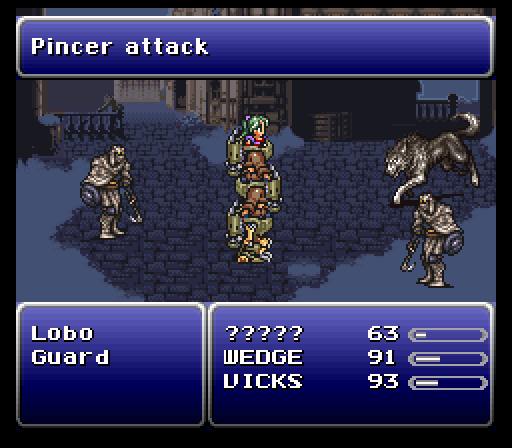
\includegraphics[width=0.5\textwidth]{pincer.png}

\end{frame}

\begin{frame}
\frametitle{Attacking from both sides}

Why do these algorithms (Jump Pointers and Ladders) work?

\pause\vspace{1em}
Jump pointers allow us to cover a lot of ground quickly: at least half the
distance to our destination in the first step.

\pause\vspace{1em}
Ladders start out slowly, but once you're halfway to the destination, you
get there in one more jump.

\end{frame}

\begin{frame}
\frametitle{Attacking from both sides}

\begin{block}{Preprocessing}
  Construct both the jump pointers and the ladder decomposition of $T$.
\end{block}

\pause

\begin{block}{Query}
  Consider $LA_T(\nu, d)$.  We need to travel up
  $\delta = Depth(\nu) - d$.

  \pause\vspace{1em} One step of the jump pointer algorithm takes us to a
  node $\nu'$ at least $\delta/2$ higher than $\nu$.

  \pause\vspace{1em} This node $\nu'$ has height $h' \ge \delta/2$.  The
  ladder for $\nu'$ must extend higher by at least another $h'$, which is
  enough to take us the rest of the way.
\end{block}

\end{frame}

\begin{frame}
\frametitle{Attacking from both sides \visible<3->{$\left<O(n\log n), O(1)\right>$}}

\begin{block}{Preprocessing}
  Jump pointers cost $O(n\log n)$ preprocessing, and the ladder
  decomposition costs $O(n)$.
\end{block}

\pause

\begin{block}{Query}
  We need to follow one jump pointer ($O(1)$) and use one ladder ($O(1)$).
\end{block}

\end{frame}

\begin{frame}
\frametitle{Recap}

We have a data structure that lets us travel up the tree to arbitrary
depth in constant time, and is built in $O(n\log n)$ time.

\pause\vspace{1em}

Now let's build it in linear time.

\end{frame}

\begin{frame}
\frametitle{}

\centering
\Large
Mathematicians HATE me for this one weird trick...

\end{frame}

\subsection{Optimal Result}

\begin{frame}
\frametitle{One weird math trick...}

Consider a problem of size $n$.

\pause We will divide this into $O(n/\log n)$ subproblems each of size
$O(\log n)$, and one superproblem of size $O(n/\log n)$.

\pause We'll use an $O(n\log n)$ algorithm to solve the superproblem, and
then we just have small problems left to solve, which we'll also solve
quickly.

\end{frame}

\begin{frame}
\frametitle{One weird math trick...}

Let $m = O(n/\log n)$ be the size of the superproblem.

The preprocessing complexity for the superproblem is:
\pause
\begin{equation*}
\begin{split}
  O(m\log m) &= O\left( \frac{n}{\log n} \log \left( \frac{n}{\log n} \right) \right) \\
  \visible<3->{&= O\left( \frac{n}{\log n} \left( \log n - \log\log n \right) \right)} \\
  \visible<4->{&= O\left( \frac{n}{\log n} \log n \right)} \visible<6->{= O\left( n \right)}
\end{split}
\end{equation*}

\end{frame}

\begin{frame}
\frametitle{Macro-Micro-Tree Algorithm}

\begin{columns}[onlytextwidth]
  \begin{column}{.58\textwidth}

    We choose \alert{Jump Nodes} as the maximally deep nodes with at least
    $\log(n)/4$ descendants

    \vspace{1em}
    \visible<3->{
      This gives us many ``micro trees'' of size less than $\log(n)/4$,
      and one ``macro tree'' of size $O(n/\log n)$.  The macro tree has
      the jump nodes as its leaves.
    }

    \vspace{1em}
    \visible<4->{
      We compute jump pointers only for these jump nodes, and for all
      other nodes $\nu$ in the macro tree, we assign $JumpDesc(\nu)$ to be
      one of its jump node descendants.
    }

  \end{column}%
  \hfill%
  \begin{column}{.38\textwidth}

    \begin{figure}
      \centering
      \begin{tikzpicture}[
        node distance = 0.1cm, sibling distance = 5mm, level distance = 5mm,
        every node/.style={black,circle,draw,fill=black,scale=0.5},
        subtree/.style={black,isosceles triangle,shape border rotate=90,draw,fill=white,scale=1.0}
        ]
        \node {}
        [child anchor=north]
        child {
          node (x) {}
          child {
            node {}
            child {
              node[onslide=<2->{red}] (y) {}
              child {
                node[subtree] {}
              }
            }
            child {
              node[subtree] {}
            }
          }
          child {
            node[onslide=<2->{red}] {}
            child {
              node[subtree] {}
            }
          }
        }
        child[missing]
        child {
          node {}
          child {
            node {}
            child {
              node[subtree] {}
            }
            child {
              node[onslide=<2->{red}] {}
              child {
                node[subtree] {}
              }
              child {
                node[subtree] {}
              }
            }
          }
        }
        child[missing]
        child {
          node (z) {}
          child {
            node {}
            child {
              node[onslide=<2->{red}] {}
              child {
                node[subtree] {}
              }
            }
          }
          child {
            node[onslide=<2->{red}] (w) {}
            child {
              node[subtree] {}
            }
            child {
              node[subtree] {}
            }
          }
        } ;
        \path[->,>=stealth,onslide=<5>{purple},onslide=<-4>{white}]
        (x) edge [bend right] (y)
        (z) edge [bend left] (w) ;
        \tikzstyle{every node}=[]
      \end{tikzpicture}
    \end{figure}

  \end{column}%
\end{columns}

\end{frame}

\begin{frame}
\frametitle{Macro-Micro-Tree Algorithm}

\begin{columns}[onlytextwidth]
  \begin{column}{.58\textwidth}

    To solve a query $LA_T(\nu, d)$ where $\nu$ is in the macro tree, we
    first jump down to $JumpDesc(\nu)$, then use one of its jump pointers
    and then one ladder to find $LA_T(JumpDesc(\nu), d) = LA_T(\nu, d)$.

  \end{column}%
  \hfill%
  \begin{column}{.38\textwidth}

    \begin{figure}
      \centering
      \begin{tikzpicture}[
        node distance = 0.1cm, sibling distance = 5mm, level distance = 5mm,
        every node/.style={black,circle,draw,fill=black,scale=0.5},
        subtree/.style={black,isosceles triangle,shape border rotate=90,draw,fill=white,scale=1.0}
        ]
        \node {}
        [child anchor=north]
        child {
          node {}
          child {
            node {}
            child {
              node[red] {}
              child {
                node[subtree] {}
              }
            }
            child {
              node[subtree] {}
            }
          }
          child {
            node[red] {}
            child {
              node[subtree] {}
            }
          }
        }
        child[missing]
        child {
          node {}
          child {
            node {}
            child {
              node[subtree] {}
            }
            child {
              node[red] {}
              child {
                node[subtree] {}
              }
              child {
                node[subtree] {}
              }
            }
          }
        }
        child[missing]
        child {
          node {}
          child {
            node {}
            child {
              node[red] {}
              child {
                node[subtree] {}
              }
            }
          }
          child {
            node[red] {}
            child {
              node[subtree] {}
            }
            child {
              node[subtree] {}
            }
          }
        } ;
        \tikzstyle{every node}=[]
      \end{tikzpicture}
    \end{figure}

  \end{column}%
\end{columns}

\end{frame}

\begin{frame}
\frametitle{Macro-Micro-Tree Algorithm}

\begin{columns}[onlytextwidth]
  \begin{column}{.58\textwidth}

    If the query is in one of the micro trees, we need a strategy to solve it.

    \vspace{1em}

    \visible<2->{
      Consider a DFS on a micro tree.  We visit each edge twice, first
      going down, then later, going up.
    }

    \vspace{1em}

    \visible<2->{
      We can identify a tree shape with $m$ nodes with a bit vector,
      representing the DFS, of length $2(m-1)$.
    }

    \vspace{1em}

    \visible<11->{
      Each micro tree has less than $\log(n)/4$ nodes, so there are few
      possible shapes of micro tree:
    }
    \visible<12->{
      \[
      2^{2(m-1)} \le 2^{\log(n)/2} = \left( 2^{\log n} \right)^{\frac 1 2} = \sqrt n
      \]
    }

  \end{column}%
  \hfill%
  \begin{column}{.38\textwidth}

    \begin{figure}
      \centering
      \begin{tikzpicture}[
        node distance = 0.1cm, sibling distance = 10mm, level distance = 10mm,
        every node/.style={black,circle,draw,fill=white},
        ]
        \node (a) {}
        child {
          node (b) {}
          child {
            node (c) {}
          }
          child {
            node (d) {}
          }
        } 
        child {
          node (e) {}
        } ;
        \path[->,>=stealth]
        (a) edge [bend right,onslide=<-2>{white},onslide=<3->{red}] (b)
        (b) edge [bend right,onslide=<-3>{white},onslide=<4->{orange}] (c)
        (b) edge [bend right,onslide=<-5>{white},onslide=<6->{ForestGreen}] (d)
        (c) edge [bend right,onslide=<-4>{white},onslide=<5->{YellowOrange}] (b)
        (d) edge [bend right,onslide=<-6>{white},onslide=<7->{TealBlue}] (b)
        (a) edge [bend right,onslide=<-8>{white},onslide=<9->{violet}] (e)
        (b) edge [bend right,onslide=<-7>{white},onslide=<8->{airforceblue}] (a)
        (e) edge [bend right,onslide=<-9>{white},onslide=<10->{purple}] (a) ;
        \tikzstyle{every node}=[]
      \end{tikzpicture}
    \end{figure}

    \visible<3->{
      \begin{figure}
        \centering
        \begin{tabular}{|c|c|c|c|c|c|c|c|}
          \hline
          \visible<3->{\color{red} 0}
          & \visible<4->{\color{orange} 0}
          & \visible<5->{\color{YellowOrange} 1}
          & \visible<6->{\color{ForestGreen} 0} 
          & \visible<7->{\color{TealBlue} 1}
          & \visible<8->{\color{airforceblue} 1}
          & \visible<9->{\color{violet} 0} 
          & \visible<10->{\color{purple} 1} \\
          \hline
        \end{tabular}
      \end{figure}
    }

  \end{column}%
\end{columns}

\end{frame}

\begin{frame}
\frametitle{Macro-Micro-Tree Algorithm}

We'll use the simple $\left<O(n^2), O(1)\right>$ Table Algorithm to
preprocess \textbf{every possible} micro tree shape.

\pause\vspace{1em}

To answer a query $LA_T(\nu, d)$ when $\nu$ is in a micro tree, either:
\begin{itemize}
\item Use the Table Algorithm if the target is in the micro tree.
\item Jump to the root of the micro tree and use the macro tree algorithm
  from its parent.
\end{itemize}

\end{frame}

\begin{frame}
\frametitle{Macro-Micro-Tree Algorithm}

\begin{block}{Preprocessing}
  As before, we can build the Ladder Algorithm's data structure in $O(n)$
  time.

  \pause\vspace{1em} We can identify the jump nodes and the micro trees
  with DFS.

  We can compute jump pointers for the jump nodes, using the ladders, in
  $O(\log n)$ time per jump node.  There are $O(n/\log n)$ jump nodes, so
  computing all jump pointers takes $O(n)$ time.

  \pause\vspace{1em} Preprocessing one micro tree costs $O(\log^2 n)$, so
  all microtrees together have complexity $O(\sqrt n \log^2 n) \le O(n)$.

\end{block}

\end{frame}

\begin{frame}
\frametitle{Macro-Micro-Tree Algorithm \visible<3->{$\left< O(n), O(1) \right>$}}

\begin{block}{Query}
  If the query is in the macro tree, we jump down to a jump node, use one
  jump pointer, and one ladder, which are all $O(1)$.

  \pause\vspace{1em} If the query is in the micro tree, we solve it there
  with the Table Algorithm in $O(1)$ time, or use the macro tree, which is
  also $O(1)$ as above.
\end{block}

\end{frame}

\begin{frame}
\frametitle{Lessons}

\begin{itemize}
\item<2-> Look for paired algorithms that complement each other by reinforcing
  each others' weaknesses (Ladders and Jump Pointers).
\item<3-> Turn an $O(n\log n)$ algorithm into an $O(n)$ algorithm:
  \begin{itemize}
  \item<4-> Divide into subproblems of size $O(\log n)$ which are easier
    to solve together.

    Usually, you want to find duplicates.
  \item<5-> Solve the $O(n/\log n)$ problem instance with the fancy
    algorithm.
  \item<6-> PWL NYC \#7: {\em The LCA Problem Revisited}
    (\href{https://bit.ly/pwl-lca}{bit.ly/pwl-lca})
  \end{itemize}
\end{itemize}

\end{frame}

\section{Thanks}

\begin{frame}
\frametitle{}

\centering
\Large
Thanks!

\end{frame}

\end{document}
